
\documentclass[journal]{IEEEtran}
% \documentclass[conference]{IEEEtran
\IEEEoverridecommandlockouts
% The preceding line is only needed to identify funding in the first footnote. If that is unneeded, please comment it out.
\usepackage{cite}
\usepackage[margin=1in]{geometry}
\usepackage{amsmath,amsthm,amssymb}
\usepackage{algorithmic}
\usepackage{graphicx} 
\graphicspath{{./figures/}{../png/} }
\usepackage{subfig}
\usepackage{wrapfig}
\def\BibTeX{{\rm B\kern-.05em{\sc i\kern-.025em b}\kern-.08em
    T\kern-.1667em\lower.7ex\hbox{E}\kern-.125emX}}

% This is to include code
\usepackage{listings}
\usepackage{xcolor}
\definecolor{dkgreen}{rgb}{0,0.6,0}
\definecolor{gray}{rgb}{0.5,0.5,0.5}
\definecolor{mauve}{rgb}{0.58,0,0.82}
\lstdefinestyle{Python}{
    language        = Python,
    basicstyle      = \ttfamily,
    keywordstyle    = \color{blue},
    keywordstyle    = [2] \color{teal},
    stringstyle     = \color{green},
    commentstyle    = \color{red}\ttfamily}

\newcommand{\N}{\mathbb{N}}
\newcommand{\Z}{\mathbb{Z}}

\newenvironment{theorem}[2][Theorem]{\begin{trivlist}
\item[\hskip \labelsep {\bfseries #1}\hskip \labelsep {\bfseries #2.}]}{\end{trivlist}}
\newenvironment{lemma}[2][Lemma]{\begin{trivlist}
\item[\hskip \labelsep {\bfseries #1}\hskip \labelsep {\bfseries #2.}]}{\end{trivlist}}
\newenvironment{exercise}[2][Exercise]{\begin{trivlist}
\item[\hskip \labelsep {\bfseries #1}\hskip \labelsep {\bfseries #2.}]}{\end{trivlist}}
\newenvironment{reflection}[2][Reflection]{\begin{trivlist}
\item[\hskip \labelsep {\bfseries #1}\hskip \labelsep {\bfseries #2.}]}{\end{trivlist}}
\newenvironment{proposition}[2][Proposition]{\begin{trivlist}
\item[\hskip \labelsep {\bfseries #1}\hskip \labelsep {\bfseries #2.}]}{\end{trivlist}}
\newenvironment{corollary}[2][Corollary]{\begin{trivlist}
\item[\hskip \labelsep {\bfseries #1}\hskip \labelsep {\bfseries #2.}]}{\end{trivlist}}

\hyphenation{op-tical net-works semi-conduc-tor}

%% For our reference part
%\makeatletter
%\def\bstctlcite{\@ifnextchar[{\@bstctlcite}{\@bstctlcite[@auxout]}}
%\def\bstctlcite[#1]#2{\@bsphack\@for\@citeb:=#2\do{%
%\edef\@citeb{\expandafter\@firstofone\@citeb}%
%\if@filesw\immediate\write\csname #1\endcsname{\string\citation{\@citeb}}\fi}
%\@esphack}
%\makeatother

\begin{document}
%\bstctlcite{IEEEexample:BSTcontrol}

% --------------------------------------------------------------
%                         Start here
% --------------------------------------------------------------

\title{MIALab Project HS2020 - \\ Image normalization has an important influence on the segmentation}

\author{\IEEEauthorblockN{Thomas Buchegger} \IEEEauthorblockA{\textit{University of Bern,}}
\and \IEEEauthorblockN{Carolina Duran} \IEEEauthorblockA{\textit{University of Bern,}}
\and \IEEEauthorblockN{Stefan Weber,} \IEEEauthorblockA{\textit{University of Bern}}
\thanks{T. Buchegger, C. Duran and S. Weber are students from the University of Berne in Switzerland.}%
\thanks{E-mail of T. Buchegger: thomas.buchegger@students.unibe.ch}%
\thanks{E-mail of C. Duran: carolina.duran@students.unibe.ch}%
\thanks{E-mail of S. Weber: stefan.weber1@students.unibe.ch}}

\markboth{MIALab Project HS2020, January~2021}%
{Buchegger, Duran and Weber: Image normalization has an important influence on the segmentation}
\maketitle
%\pagestyle{plain}
\newpage


% --------------------------------------------------------------
% Abstract
% --------------------------------------------------------------

\begin{abstract}
Here is the abstract.


\end{abstract}
\hfill January 03, 2021



% --------------------------------------------------------------
% Introduction
% --------------------------------------------------------------

\section{Introduction}

	This is a very important citation test. \cite{Roohani2018}	
	Postprocesses of clinical diagnosis images for treatment planning often include manual segmentation of brain regions. 
	To segment and label the brain structures in a large dataset is complicated and time-consuming by manual operator-guided segmentation. 
	Furthermore, it is affected by user variability and prone to limiting the standardisation. 
	This paper will depend upon automated segmentation that segments and labels five different brain regions. \\


	To conclude we hypothesis that normalization has an important influence in the segmentation process of brain regions. 
	We present in this paper the acquired results applying multiple normalization methods and comparing them for every segmented brain region. 
	Furthermore, we analyse the results and conclude our findings. \\


\textbf{Our hypothesis: "Image normalization has an important influence on the segmentation".
	Aims of the introduction:
	\begin{itemize}
	\item To demonstrate importance/impact need
	\item To demonstrate novelty
	\item To justify the hypothesis / aims / investigated technology
	\item To establish expectations/scope of the report
	\end{itemize} 
	Some questions which could be answered:
	Currently, z score normalization is implemented.
	\begin{itemize}
	\item Are there more powerful normalization methods?
	\item Is normalization really needed?
	\item Is the provided data already normalized in some way?
	\item Can you also unnormalize data to show a negative effect?
	\end{itemize}
	For the research:
	\begin{itemize}
	\item Understand the problem
	\item What have others already done / is there already a solution?
	\item Can I apply a solution to another problem to my problem?
	\item What lessons can I learn from others work?
	\item What deficiencies exist in others work?
	\end{itemize}
	\begin{enumerate}
	\item Demonstrate importance
		\begin{enumerate}
		\item Define the problem
		\item Explain the criticality, impact of the problem
		\end{enumerate}
	\item Demonstrate Novelty
		\begin{enumerate}
		\item Explain what is the state of the art / current practice
		\item Explain what preliminary / related work has been done towards solving the problem by you and others
		\item Explain what deficiencies / problems still exist (specifically the one that you will try to address)
		\end{enumerate}
	\item Present and Justify the Hypothesis / aim / objective
		\begin{enumerate}
		\item State Hypothesis /aim/ objective
		\item Describe evidence supporting hypothesis
		\end{enumerate}
	\item Establish expectations of the report
		\begin{enumerate}
		\item Describe scope of the presented work
		\item Present a summary of remainder of the report\\
		\end{enumerate}
	\end{enumerate} 
}


% --------------------------------------------------------------
% Materials & Methods
% --------------------------------------------------------------

\section{Materials and Methods}
\textbf{MIA pipeline in general (short overview ), your experiment in detail}
\subsection{Medical Backgrund}
	The five brain regions segmented in this paper are the white and grey matter, hippocampus, amygdala and the thalamus. All regions are visible in figure \ref{fig:e1}.

	% --------------------------------------------------------------
	\begin{figure}[h]
		\centering
		%omit extension of file. pdflatex will convert to pdf automatically.
		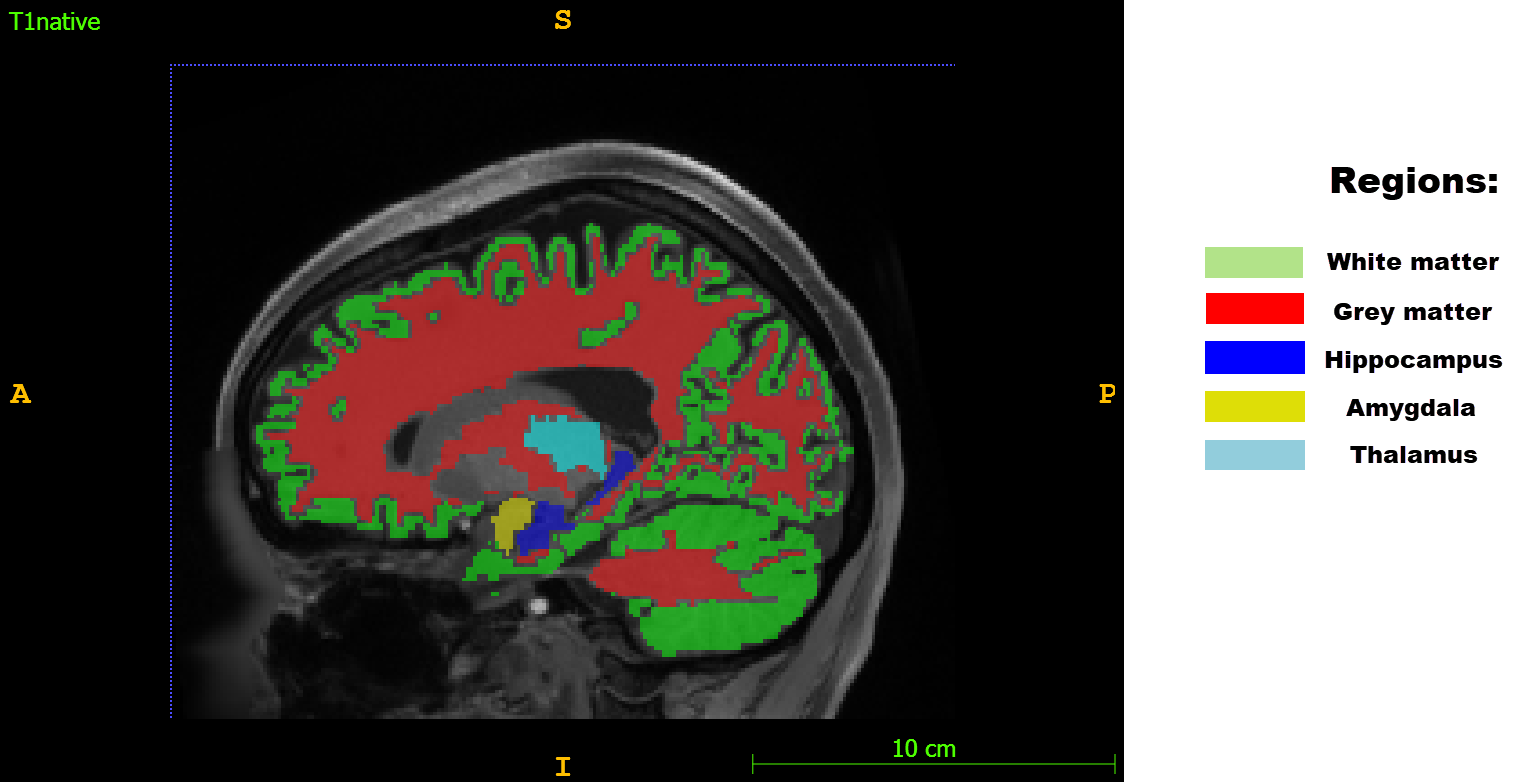
\includegraphics[width=0.4\textwidth]{T1native_all_regions_labelled}
		\caption{The five brain regions which are segmented and labelled.}
		\label{fig:e1}
	\end{figure}
	% --------------------------------------------------------------

\subsection{Data}
	The data we used was provided by the Medical Image Analysis Lab team at the University of Bern. Overall, our dataset consists of 32 MRI,
	out of which 21 we used for training and 11 for testing our model. From each patient we have a T1-weighted and a T2-weighted image. Each MRI file
	is of the size 118x118x217.
\subsection{Model}
	The model we used is a Random Forest classifier with which we combined different parameters with all used normalization techniques. Which parameters
	lead to which result can be found in the results section. For normalization techniques, we used the following:
	\begin{itemize}
		\item zScore
		\begin{equation}
			z = \frac{x - \mu}{\sigma}
		\end{equation}
		\item minMax
		\begin{equation}
			z = \frac{x - x_{min}}{x_{max} - x_{min}}
		\end{equation}
		\item stikN
		\item Whitestripe
		\item Fuzzy-C means\\
		With fuzzy c-means we find a mask for a specified tissue type given a T1w image and its brain mask. Create a tissue mask
		from that T1w image's FCM tissue mask. Then we can use that tissue mask as input to the func again, where the tissue mask is
		used to find an approximate mean of the tissue intensity in	another target contrast, and move it to some standard value.
		\item Histogram Matching
		\item Gaussian Mixture Model
	\end{itemize}
\subsection{Evaluation}
	For this paper, we evaluated our used normalization techniques on our inhouse T1-weighted and T2-weighted MRI data sets. 
	We chose the Dice Similarity Coefficient (DCS) as well as the Hausdorff distance to evaluate the different normalization techniques.
	Dice Similarity Coefficient returns as a quality metric how much two regions overlap and is, therefore, a useful metric for segmentation.
	The dice coefficient of two sets, as explained in figure \ref{fig:e2}, is a measure of their intersection scaled by their size. The result is in the range from 0 to 1, where 1 is a perfect segmentation. 
	
	% --------------------------------------------------------------
	\begin{figure}[h]
		\centering
		%omit extension of file. pdflatex will convert to pdf automatically.
		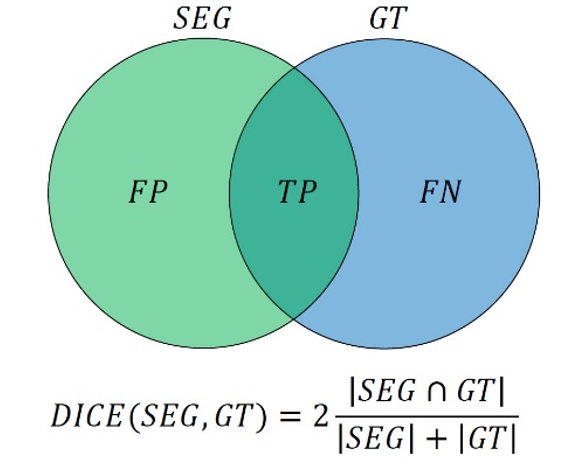
\includegraphics[width=0.4\textwidth]{diceGraphics}
		\caption{Graphical representation of the Dice Similarity Coefficien. SEG stands for the achieved segmentation whereas GT means ground truth.}
		\label{fig:e2}
	\end{figure}
	% --------------------------------------------------------------

	The Hausdorff distance measures how far two subsets of a metric space are from each other. So two sets are close if every point of either set is close 
	to some point of the other set. Then the Hausdorff distance, explained in figure \ref{fig:e3}, is the longest distance from one of the two sets to the other set.

	% --------------------------------------------------------------
	\begin{figure}[h]
		\centering
		%omit extension of file. pdflatex will convert to pdf automatically.
		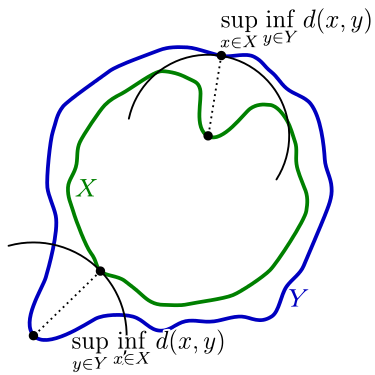
\includegraphics[width=0.4\textwidth]{haussdorfGraphics}
		\caption{Components of the calculation of the Hausdorff distance between the green line X and the blue line Y.}
		\label{fig:e3}
	\end{figure}
	% --------------------------------------------------------------


% --------------------------------------------------------------
% Results
% --------------------------------------------------------------

\section{Results}
\textbf{In depth analysis of experiment related results}

\subsection{Data}
\subsection{Model}
\subsection{Evaluation}

% --------------------------------------------------------------
% Discussion
% --------------------------------------------------------------

\section{Discussion}
\textbf{Aims of the Discussion part:
\begin{itemize}
\item Highlight importance of your work (highlight novelty /impact etc
\item To interpret your results in relation to your original problem
\item To put your work into the context of existing work
\item To present any limitations of the presented work
\item To make future recommendations
\item To provide a conclusion of the work
\end{itemize}
\begin{enumerate}
\item Importance of the work
	\begin{enumerate}
	\item Summarise your results
	\item Reiterate the importance of the work (novelty , impact etc)
	\end{enumerate}
\item Interpretation of results
	\begin{enumerate}
	\item Interpret your results focussing on the problem described in the introduction. What do the results mean for the described problem?
	\item Explain any unusual/important findings (be careful if not your original investigative subject)
	\end{enumerate}
\item Provide context
	\begin{enumerate}
	\item Describe your results in relation to others and try to explain any discrepancies
	\item Emphasize how your results support or refute your hypotheses current thinking in the field. Were results as expected? If not why and what does this mean?
	\end{enumerate}
\item Limitations of your work
	\begin{enumerate}
	\item Describe any limitations /deficiencies of your work and what impact they have on the findings
	\item Suggest possible future solutions
	\end{enumerate}
\end{enumerate} 
}

% --------------------------------------------------------------
% Conclusion
% --------------------------------------------------------------

\section{Conclusion}
\textbf{	
	\begin{itemize}
	\item Summarise your findings and relate your findings back to your hypothesis / aim / objective and to your problem.
	\item Based on your findings, suggest next steps towards solving your problem
	\end{itemize}
}
\pagebreak

% --------------------------------------------------------------
% References
% --------------------------------------------------------------

\bibliographystyle{ieeetr}
\bibliography{MIALab} 

\end{document}
